{
\section{Suitable title}
Let $\xi_\epsilon=(X,Y,\epsilon)$ be a couple of $\epsilon$-resampled
Brownian webs as defined in \FIXME{a earlier section}{definition section come here}. We denoted by $e_\epsilon(t)$ a
sample of $\xi_\epsilon$ starting at some given point at time
$0$. $x(t)$ will denote a sample of $X$ starting at the same
point. Our goal in this section is to prove the following theorem:

\begin{theorem}\label{thm:main1}
Under the previous notations, $\ds\lim_{\epsilon \rightarrow 0}
|e_\epsilon(1)- x(1)| = 0$ where the convergence is in probability.
\end{theorem}

In order to prove this it will be easier to prove the following
stronger claim:
\begin{theorem}\label{thm:main2}
For every $t\in[0,1]$ and every $\delta>0$ it is true that
$$\ds lim_{\epsilon \rightarrow 0}P\left(\text{either } x(t)=e_\epsilon(t)
\text{ or }x(t)^2+\frac{(e_\epsilon(t)-x(t))^2}{\sqrt2}<\delta\right)=1$$
Equivalently the two dimensional process $(x(t),\frac{(e_\epsilon(t)-x(t))}{\sqrt2})$
a.s. leaves the $\sqrt\delta$ ball only through
$(\sqrt\delta,0)$ or through
$(-\sqrt\delta,0)$.
\end{theorem}

One can easily see from the definition of $\epsilon$-resampled
Brownian webs that Proposition \ref{thm:main2} infers theorem
\ref{thm:main1}.

 We begin by presenting a handy theorem whose proof
we delay to subsection \ref{sec:POC}:

\begin{theorem}\label{thm:no-escape}
Suppose that on time $t_0$ we have
$e(t_0)=0$, let $t>0$ be the first time at which
$x(t)^2+\frac{(e_\epsilon(t)-x(t))^2}{\sqrt2}=1$, then the probability
that $x(t)=e_\epsilon(t)=\pm1$ is at least $1-O(\frac1{log\epsilon})$.
\end{theorem}

Applying scaling invariance to this theorem immediately yields the
following corollary:
\begin{cor}\label{cor:cor1}
Let $\delta>0$ suppose that on time $t_0$ we have $e(t_0)=(0,0)$, let
$t>0$ be the first time at which
$x(t)^2+(x(t)-\frac{(e_\epsilon(t)-x(t))^2)}{\sqrt2}=\delta$, then the probability
that $x(t)=e_\epsilon(t)=\pm\sqrt\delta$ is at least
$1-O(\frac{1}{log\epsilon/\delta})$.
\end{cor}

In order to overcome the gap between Corollary \ref{cor:cor1} and
Theorem \ref{thm:main1} we present the following property of Brownian
motion:
\begin{propos}\label{prop:prop1}
Let $\delta,\zeta>0$ and let $x(t)$ be a one dimensional Brownian
motion such that $x(0)=\delta$. There exists some $k$ such that
$\P(\min_t(x(t)=0)<\frac1k)<\zeta$.
\end{propos}

We are now ready to give a proof to proposition \ref{thm:main2}.

\begin{proof}[proof (Proposition \ref{thm:main2})]
Let $\zeta,\delta>0$. We find $\epsilon>0$ such that
$\P(|e_\epsilon(1)- x(1)|\le\sqrt\delta)<\zeta$. Let $t_1,...,t_k$ be
the set of points such that $x(t_i)=0$, and there exists a time
$t_i<t'_i<t_i+1$ such that $x(t'_i)=\pm\sqrt\delta$. By Proposition
\ref{prop:prop1}, there exists $K\in\mathbb{N}$ such that with
probability $\sqrt\zeta$ it is true that
$\sum_{i=1}^k(t_{i+1}-t'_i)\ge\frac{k}{K}$, and thus $k\le K$. If there exists
$s_i\in (t_i, t'_i)$ for which
$x(s_i)^2+\frac{(e_\epsilon(s_i)-x(s_i))^2}{\sqrt2}=\delta$ then by the definition of
$t'_i$, $x(s_i)<\sqrt\delta$. By choosing $\epsilon$ properly in
Corollary \ref{cor:cor1} this happens with probability at most
$\sqrt[2K]{\zeta}$. By the independence of the process on the intervals
$[t_i,t'_i]$ we can multiply those probabilities, getting that the
probability that there exists any $s\in[0,1]$ for which
$x(s)^2+(e_\epsilon(s)-x(s))^2=\delta$ is less then
$\sqrt\zeta$. Since those intervals are not intersecting with the
intervals $(t'_i,t_{i+1})$ we have for the chosen epsilon $\P(\exists t
| x(t)^2+(e_\epsilon(t)-x(t))^2=\delta, x(t)\neq \sqrt \delta)<\zeta$
for all $t\in(0,1)$.
\end{proof}

\subsection{Proof of convergence}\label{sec:POC}
Let $\xi_\epsilon=(X,Y,\epsilon)$ as before. We denoted by by $e_\epsilon(t)$ a sample of $\xi_\epsilon$
starting at some given point at time $0$. We also denote by $x(t)$ a
sample of $X$ starting at the same point.  In this section we prove
Theorem \ref{thm:no-escape}. Our main technical tool in doing so will
be conformal maps. We begin by introducing a few more definitions: Let
$y(t)=\frac{e_\epsilon(t)-x(t)}{\sqrt2}$, and let
$\bar{b}_\epsilon(t)=(x(t),y(t))$. Sometimes, we will omit the $\epsilon$ writing $b(t)$. We always assume $\epsilon$
to be sufficiently small. We can now rephrase Theorem
\ref{thm:no-escape} as:

\begin{propos}[Theorem \ref{thm:no-escape} rephrased]\label{prop:reph}
Suppose that on time $t_0$ we have
$\bar{b}(0)=(0,0)$, let $t_1>0$ be the first time at which
$||b(t_1)||_2=1$, then the probability that $y(t_1)\neq0$ is less then
$O(\frac1{log\epsilon})$.
\end{propos}

We define the following indicator function
$A(t):=(y(t)=0)\wedge(|x(t)|>\epsilon)$. Note that whenever $A(t)=1$,
we can regard $b(t)$ as a one dimensional Brownian motion on the
$x$-axis, while whenever $A(t)=0$ we can regard it as a two
dimensional Brownian motion. We can now treat the sampled
process $b_\epsilon(t)$ as a state machine with $4$ states
$a_0,a^r_1,a_{\text{win}},a_{\text{lose}}$, one of which ($a^r_1$) has a parameter $r$.

The states are defined in the following way:
\begin{enumerate}
\item\label{n1} $b_\epsilon(t)$ is in state $a_0$ whenever $A(t)=0$.
\item\label{n2} $b_\epsilon(t)$ is in state $a^r_1$ whenever $A(t)=1$ and $|x(sup_{s<t}(A(s)=0))|=r$.
\item\label{n3} $b_\epsilon(t)$ is in state $a_\text{win}$ whenever $b_\epsilon(t)=(1,0)$.
\item\label{n4} $b_\epsilon(t)$ is in state $a_\text{lose}$ whenever $b_\epsilon(t)\neq(1,0)$ yet $||e(t)||_2=1$.
\end{enumerate}

By this definition at time $0$ our state machine is in state $a_0$,
and what we need to prove is that its probability to get to
 state $a_\text{lose}$ before getting to $a_\text{win}$ is $O(\frac1{log\epsilon})$.
 We do this by calculating the transition functions of
 this state machine. This calculation is describe by the following proposition,
 while the state machine is depicted in Figure \ref{fig:state_machine}.

 \begin{figure}[htb]
\begin{center}
\leavevmode
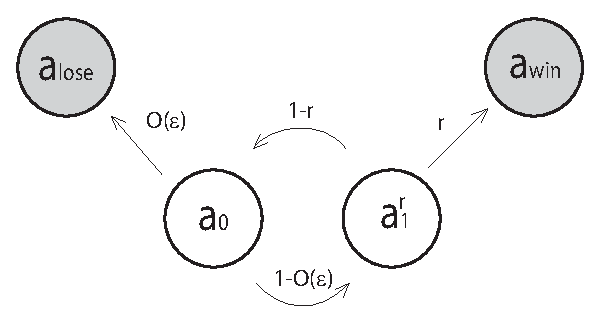
\includegraphics{state_machine.eps}
\end{center}
\caption{A diagram of the state machine.}
\label{fig:state_machine}
\end{figure}

\begin{propos}[Transition probabilities]\label{prop:trans}
The following is the transition probability of the state machine described above:
\begin{enumerate}
\item\label{m11} $\P(a^r_1\rightarrow a_0)=1-r$
\item\label{m12} $\P(a^r_1\rightarrow a_\text{win})=r$
\item\label{m13} $\P(a^r_1\rightarrow a_\text{lose})=0$
\item\label{m21} $\P(a_0\rightarrow a_\text{win})=0$
\item\label{m22} $\P(a_0\rightarrow a_\text{lose})=O(\epsilon)$
\item\label{m23} $\P(a_0\rightarrow a^r_1 \text{ for some }r)=1-O(\epsilon)$
\item\label{m24} $\P(a_0\rightarrow a^r_1 \text{ such that } r_0<r<r_1)>\ds\int_{r_0}^{r_1}(\frac{c\epsilon}{r^2}-0.5)dr$ for $r_0>2\epsilon$
\end{enumerate}
$a_\text{win}$ and $a_\text{lose}$ are trap states which are assigned no transition function.
\end{propos}

\begin{proof}
 On $a^r_1$ we know $b(t)$ is a $1$-dimensional Brownian motion starting at $r$.
 We can treat the transition time of $b(t)$ from $a^r_1$ to either $a_0$ or
 $a_\text{win}$ as a stopping time for such a Browinian motion, getting
 \ref{m11} and \ref{m12} immediately. The definition of the different states
 infers \ref{m13},\ref{m21}. The proofs of \ref{m22},\ref{m23} and \ref{m24}
 are given separately in theorem \FIXME{}{put the right theorem from the integral part} in section \FIXME{}{The integral section}.
\end{proof}

Analyzing the transition probabilities described in Proposition \ref{prop:trans} we
can find the probability of reaching $a_\text{lose}$ before $a_\text{win}$ and vice versa.
 The main step towards this result is the following theorem:

\begin{propos}\label{prop:winlose1}
Let $s_1=a_0,...,s_n$ be the sequence of states of our state machine.
\begin{equation}\label{eq:losecase}
\P(s_n=a_\text{lose} \text{ and } \ds\forall_{i>1}(s_i\neq a_0))=O(\epsilon)
\end{equation}
\begin{equation}\label{eq:wincase}
\P(s_n=a_\text{win} \text{ and } \ds\forall_{i>1}(s_i\neq a_0))=\Omega(\epsilon\log\epsilon)
\end{equation}
\end{propos}

\begin{proof}
Both \eqref{eq:losecase} and \eqref{eq:wincase} are direct results of Proposition \ref{prop:trans}.
 $a_0$ can be followed only by $a_\text{lose}$ and $a_1^r$. However $a_\text{lose}$ cannot be
 reached from $a_1^r$ without passing through
 $a_\text{win}$, thus:
 $$\P(s_n=a_\text{lose} \text{ and } \ds\forall_{i>1}(s_i\neq a_0))=\P(a_0\rightarrow a_\text{lose})=O(\epsilon)$$
 where the last equality is by item \ref{m22} in Proposition \ref{prop:trans}.
 This concludes the proof of \eqref{eq:losecase}.

 In order to reach $a_\text{win}$ we must have $a_1^r$ following $a_0$, and $a_\text{win}$
  following $a_1^r$. By \TODO{Fubini}{Should be Fubini's Theorem?} this yields the following formula:
 \begin{equation}\label{eq:r1}
 \P(s_n=a_\text{win} \text{ and } \ds\forall_{i>1}(s_i\neq a_0))=\ds\int_{\epsilon}^1 f(r) \P(a^r_1\rightarrow a_\text{win}) dr
 \end{equation}
 Where $f(r)$ is the density of the random variable $r$ which gets $r$ when
 $a_0\rightarrow a^r_1$ and $0$ otherwise. Since the density of a random variable is non-negative, we get:
 \begin{equation}\label{eq:r2}
 \P(s_n=a_\text{win} \text{ and } \ds\forall_{i>1}(s_i\neq a_0))\ge\ds\int_{2\epsilon}^1 f(r) \P(a^r_1\rightarrow a_\text{win}) dr
 \end{equation}
 Applying items \ref{m24} and \ref{m12} of Proposition \ref{prop:trans} to \eqref{eq:r2}, we get:
\begin{equation}\label{eq:r3}
 \P(s_n=a_\text{win} \text{ and } \ds\forall_{i>1}(s_i\neq a_0))\ge \ds\int_{2\epsilon}^1 (\frac{c\epsilon}{r^2}-0.5)r dr = \Omega(\epsilon\log\epsilon)
\end{equation}
\end{proof}


Proposition \ref{prop:winlose1} 
\FIXME{}{I'm Here}

} 